\documentclass[a4paper,10pt]{article}
\usepackage[utf8]{inputenc}

% increase margins
\usepackage{fullpage}
\usepackage[left=1in,top=1in,right=1in,bottom=1in,headheight=3ex,headsep=3ex]{geometry}

% this puts two lines between paragraphs and no indent
\usepackage[parfill]{parskip}

% set up colors
\usepackage{array, xcolor}
\usepackage{color,hyperref}
\usepackage{graphicx}

\definecolor{torontoblue}{HTML}{00204E}
\definecolor{linkblue}{HTML}{0000FF}

% define hyperlink style
\hypersetup{colorlinks,breaklinks,
            linkcolor=linkblue,urlcolor=linkblue,
            anchorcolor=linkblue,citecolor=linkblue}


%opening
\title{Weekly Journal}
\author{Leila Uy}



\begin{document}

\maketitle

\section{Work Update}
This journal is going to be short because I have focused a lot of my time on the Literature Review.

\subsection{Code Base}
I spent some time on the code base for a serial k-means clustering algorithm in an R notebook. Since our last meeting on 
Friday, I have not touched the code because I wanted to finish my Literature Review first. Jishnu gave me an interesting 
article which provided pseudocode that will be useful when we implement our algorithm.

\begin{figure}[h!]
    \caption{Pseudocode for a serial k-means clustering from \cite{cuomo2019a}}
    \centering
    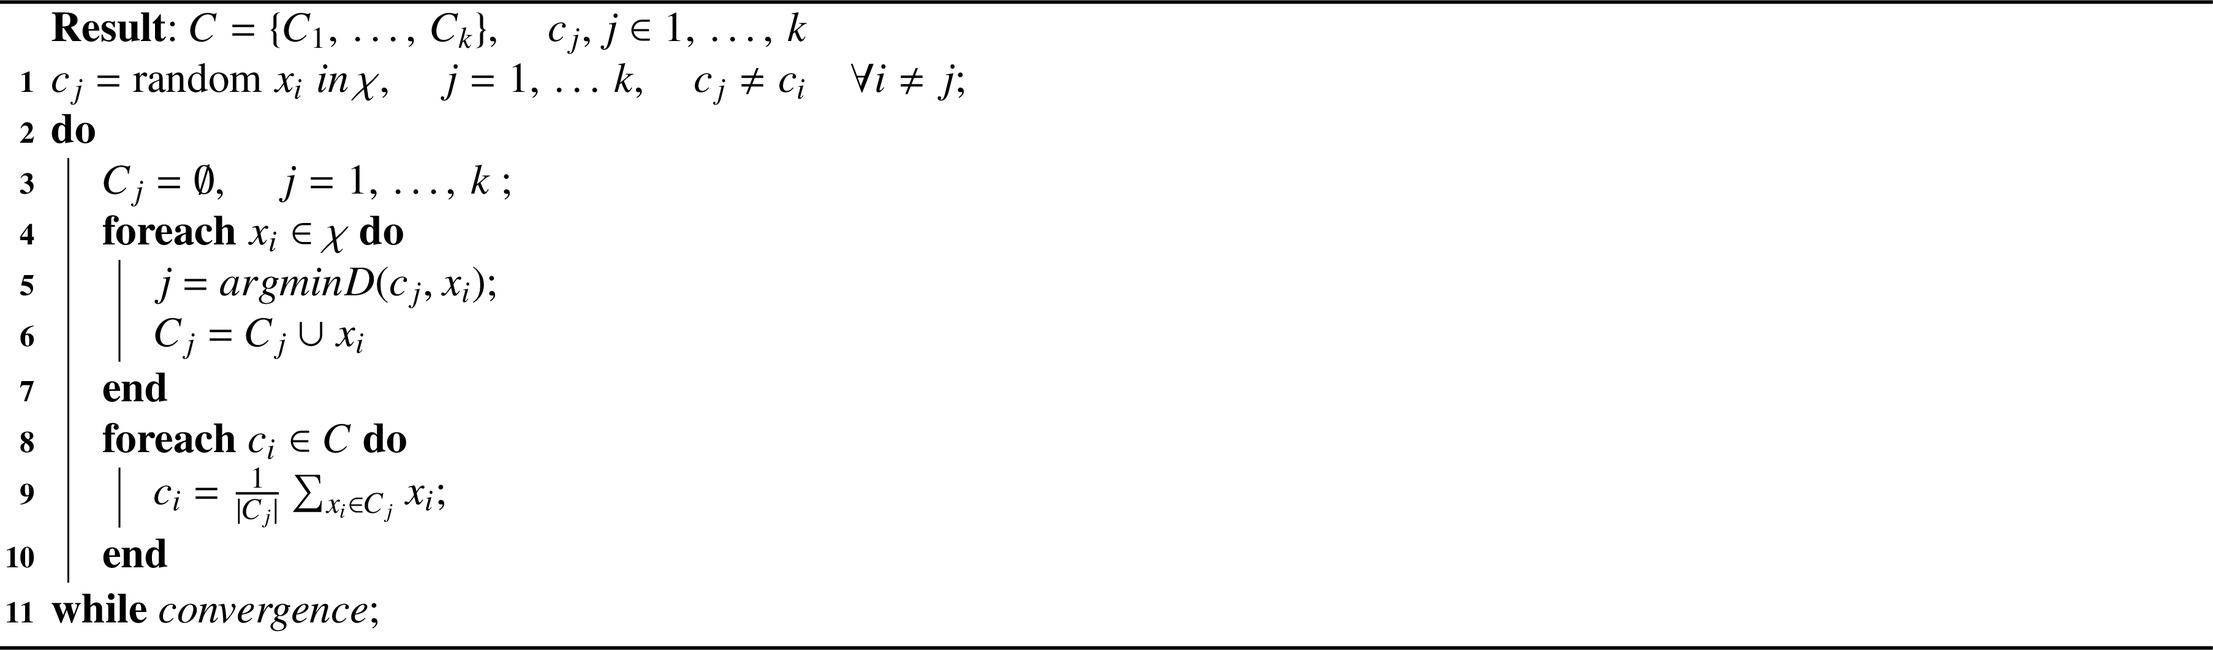
\includegraphics[scale=1.2]{code1.jpg}
\end{figure}

\begin{figure}[h!]
    \caption{Pseudocode for a parallel k-means clustering from \cite{cuomo2019a}}
    \centering
    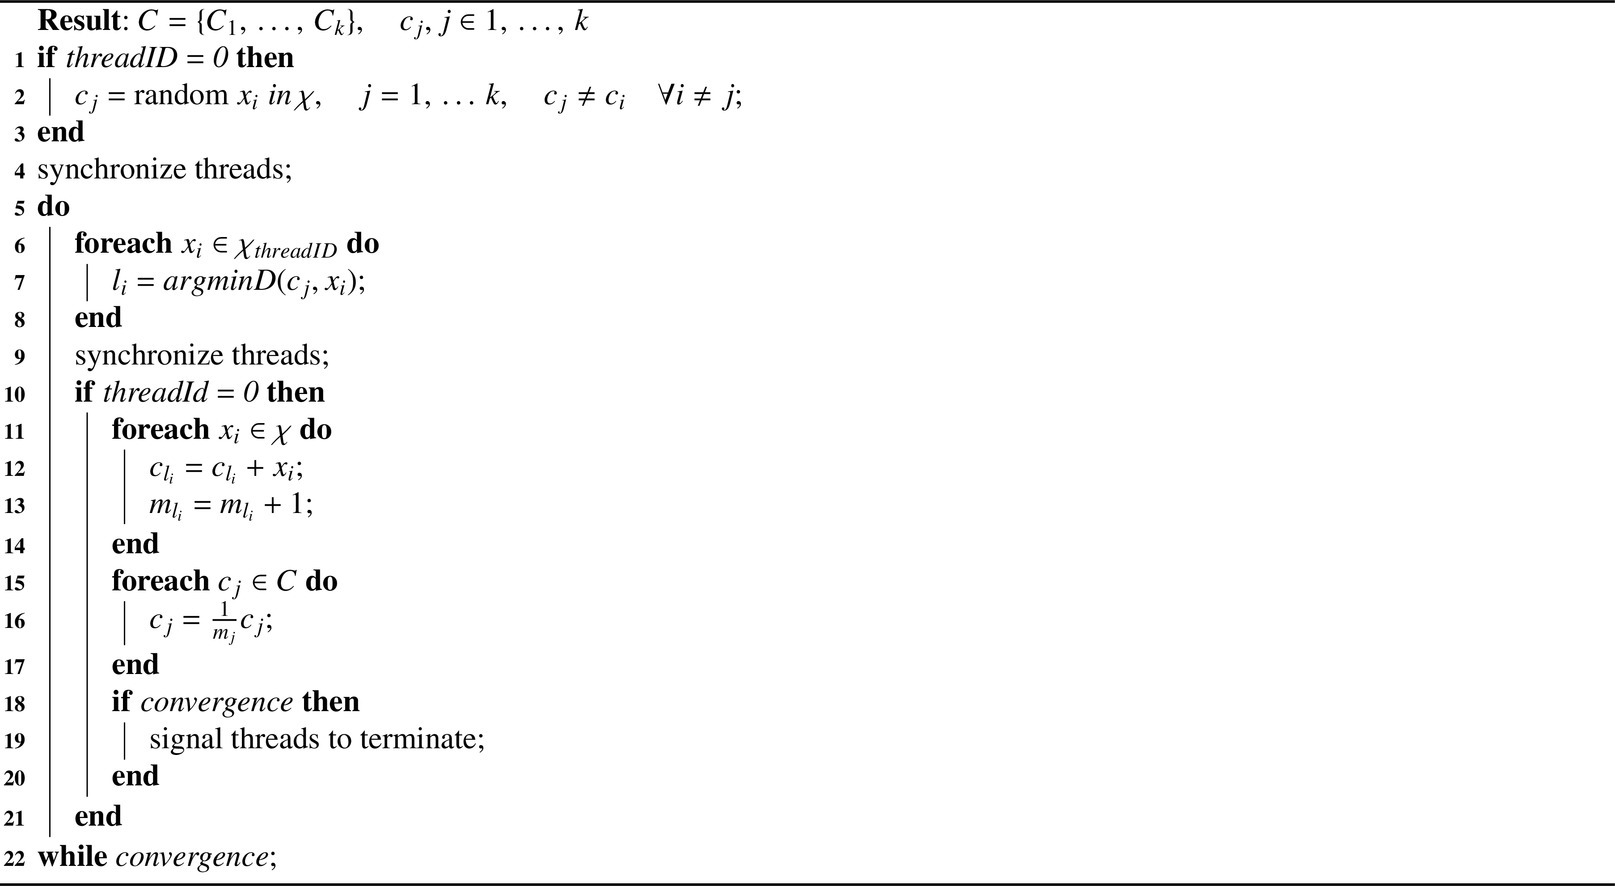
\includegraphics[scale=1.3]{code2.jpg}
\end{figure}

Currently the code uses for loops in R which I want to change to apply because it makes for more readable code and since 
apply does the for loops in C, it is slightly faster. I am also going to terminate my single processor instance on EC2 
because there is constant charges for the EBS storage even when the instance is stopped and I am going to move up to a 
4 processor instance (m4.xlarge).

For the assignment of each row of the data frame (pixel of the raster) to a cluster, I am thinking of using a format of 
dict\{clusternumber: [list of pixels]\} because it is easier to visualize with n number of variables. I think the important 
thing while implementing the clustering algorithm is to make sure that we allow for the flexibility of n number of variables 
and k number of clusters.

\section{Literature Review}
Rather than looking for new articles for my Literature Review, I looked at the citations of my old articles to expand upon 
certain points. For example, an old article I had from a previous week \cite{jain2010data}
talked about k-means clustering in great lengths and even went on to explain the different extensions of k-means clustering.
I know from the article the summary of the different extensions and what makes them unique like fuzzy c and kmeans++ but I 
wanted to go back to find the articles and skim through the papers. This means that I am able to cite them if I need to and 
I know if the algorithms are suitable for us to implement in the future \cite{dunn1973a,pelleg1999accelerating,scholkopf1998nonlinear}.

I am finished my Literature Review and Diljot, Jishnu, Valerie and I are sending our Literature Reviews to each other for 
editing on Tuesday.



% this info creates the bibliography
% YOU WILL NEED TO CHANGE THIS PATH TO THE LOCATION OF THE BIB file
\bibliography{./agclimate.bib}
\bibliographystyle{plain}


\end{document}
